\chapter{Schematy działania systemu}
\label{cha:schematy}

Pierwszym etapem symulacji było przygotowanie środowiska symulacyjnego. Na dyskretnej siatce \ref{figure:siatka}, zostali wygenerowani piesi (losowo lub nie, w zależności od parametru), przeszkody oraz punkty końcowe (wyjścia). W przypadku kiedy wyjść jest więcej niż jedno, każdemu z pieszych zostaje losowo przypisane jedno z nich. Każdemu z pieszych zostaje przypisana masa, preferowana prędkość oraz promień strefy prywatnej.
Po pełnym zainicjalizowaniu środowiska następuje wyznaczenie bazowych ścieżek przejścia dla każdego z pieszych z użyciem Algorytmu A*. Wyznaczone ścieżki służą później jako podstawa do działania SFM.
Pierwszym etapem właściwej wizualizacji jest zastosowanie SFM do obliczenia sił działających na każdego z pieszych obecnych na mapie. Po obliczeniu siły obliczone zostaje przyśpieszenie zgodnie ze wzorem \ref{eq:acc}, które służy do zaktualizowania aktualnej prędkości pieszego zgodnie z wzorem \ref{eq:predkosc}. W przypadku, gdy obliczona prędkość przekracza maksymalną, zdefiniowaną w konfiguracji, prędkość jaką może podążać pieszy zostaje ona zredukowana do dopuszczalnego poziomu. 

\begin{equation}
\label{eq:acc}
a = \frac{F}{m}
\end{equation}
gdzie:
\begin{eqwhere}[2cm]
	\item[$a$] przyśpieszanie,
	\item[$F$] siła działająca na pieszego obliczona za pomocą SFM,
	\item[$m$] masa pieszego,
\end{eqwhere}

\begin{equation}
\label{eq:predkosc}
v = v_{p} + at
\end{equation}
gdzie:
\begin{eqwhere}[2cm]
	\item[$v_{p}$] prędkość pieszego przed działaniem siły
	\item[$v$] siła po działaniu siły
	\item[$a$] przyśpieszenie
	\item[$t$] czas
\end{eqwhere}

\begin{figure}
\label{figure:siatka}
\centering
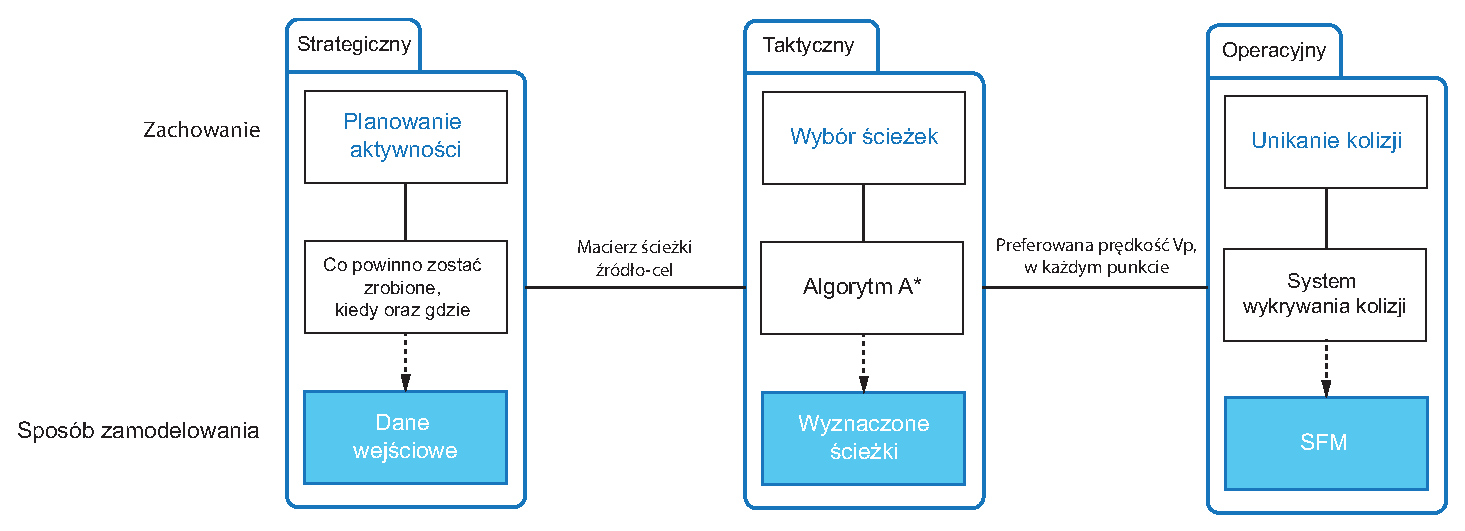
\includegraphics[width=1\textwidth]{schemat.eps}
\caption{Schemat modelu, opracowanie własne na bazie \cite{6} oraz \cite{SocialForceSuwala}}
\end{figure}

Po obliczeniu prędkości obliczana jest droga przebyta przez pieszego w każdym z kierunków. Następnie obliczony wcześniej punkt na ścieżce zostaje zmodyfikowany (lub nie np. w przypadku postoju agenta) poprzez obliczony dystans i zapisany jako aktualna pozycja danego pieszego. Wszystkie obliczone w ten sposób pozycje zostają wyświetlone na wybranej wcześniej mapie wraz z przeszkodami. Istnieje również możliwość wyświetlenia wyznaczonych na początku ścieżek za pomocą algorytmu A* oraz rzeczywistych ścieżek jakimi podążali piesi.\\
%------------
W symulacji wykorzystano ośmioelementowe sąsiedztwo Moore'a \ref{figure:siatka}. 

\begin{figure}
\label{figure:siatka}
\centering
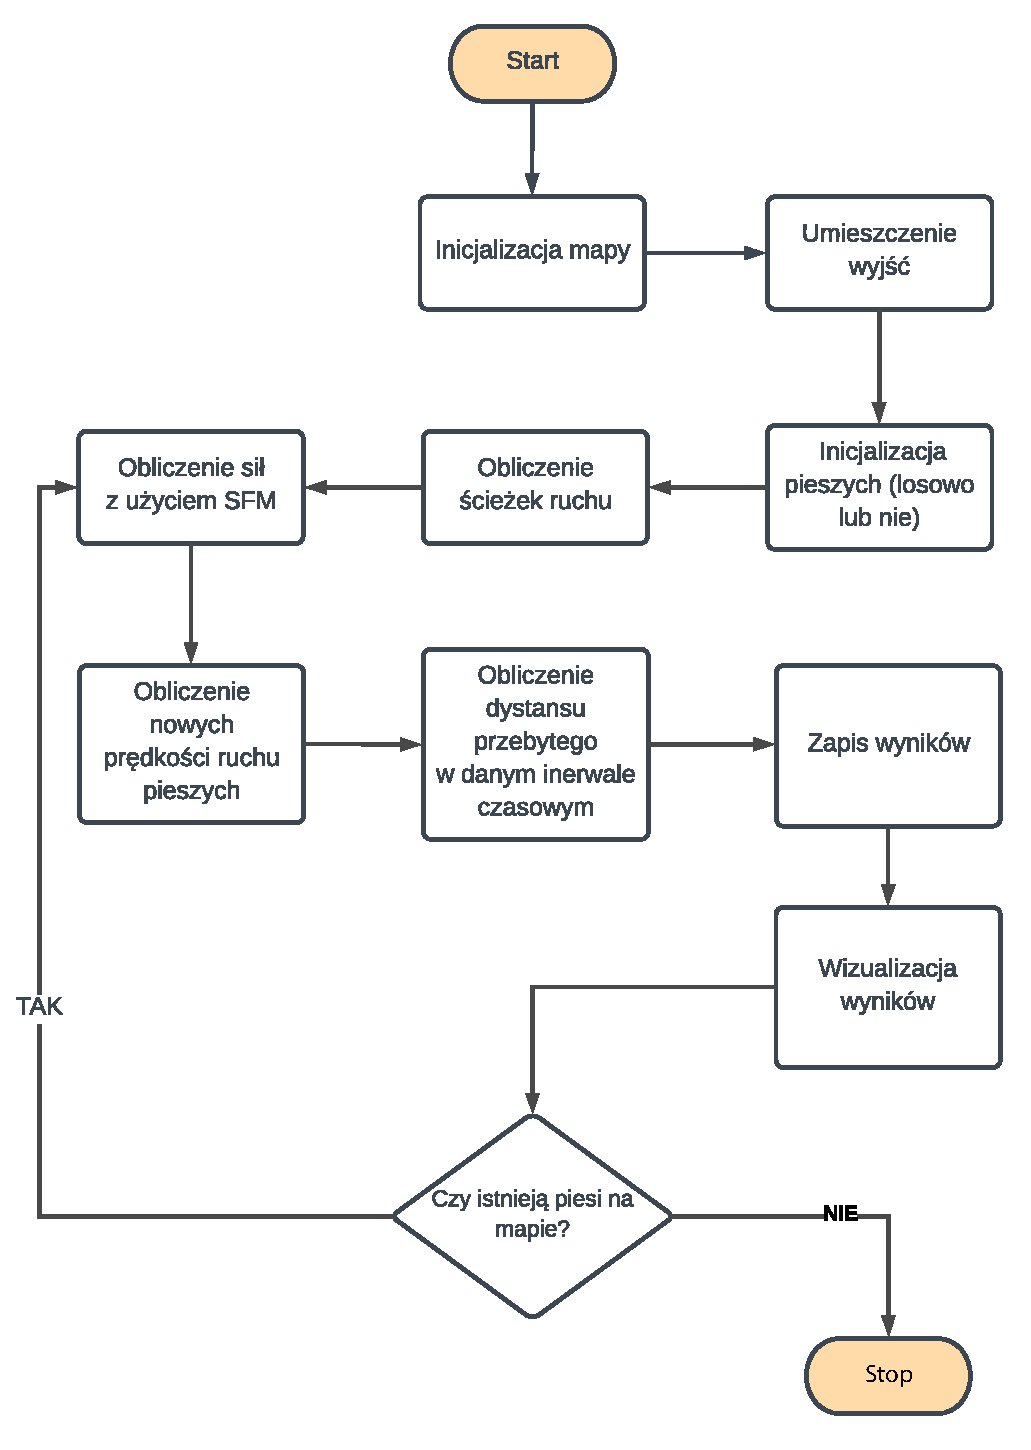
\includegraphics[width=1\textwidth]{schemat_aplikacji.eps}
\caption{Schemat działania aplikacji}
\end{figure}

\begin{figure}
\label{figure:siatka}
\centering
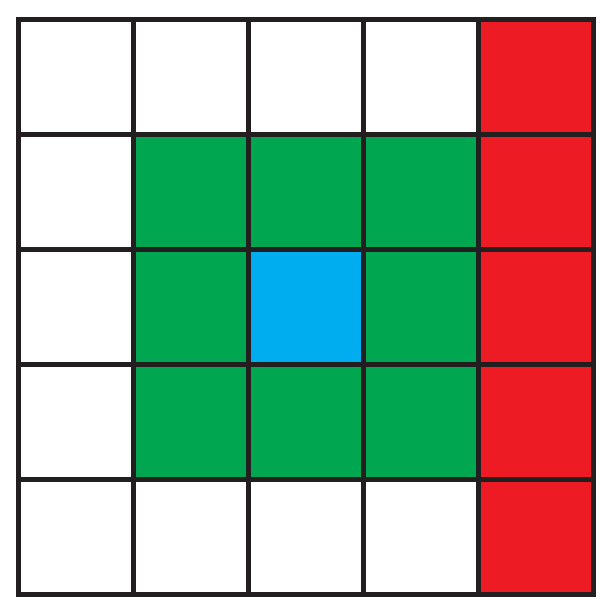
\includegraphics[width=0.4\textwidth]{sasiedztwo.eps}
\caption{Schemat siatki używanej w projekcie. Kolorem niebieskim oznaczono pieszego, zielonym jego sąsiedztwo Moore'a, czerwonym przykładowa przeszkoda}
\end{figure}

Symulacja została zaimplementowana przy użyciu języka Java w wersji 8 we wsparciu biblioteki graficznej Jwjgl.

\section{Przyjęte parametry}

Zgodnie z pracą Xiaoxia Yang \cite{GuideCrowdDynViaModifiedSocialForceModel} przyjęte zostały następujące parametry SFM:\\

\begin{center}
\begin{tabular}{c||c|c}
Symbol & Znaczenie & Wartość\\
\hline
$m$ & masa pieszego & $80kg$ \\ 
$r$ & promień strefy prywatnej & $0.25m$ \\
$A$ & Intensywność działania siły socjologicznej & $2000 N$ \\
$B$ & dytans działania siły & $0.08 m$ \\
$\kappa$ & coeficient of sliding & $240000 kg \cdot m^{-1}s^{-1}$ \\
$k$ & body coo & $120000 kg \cdot s^{-2}$ \\
$\tau$ & Czas relakasacji & $0.5 s$ \\
\end{tabular} 
\end{center}
